\documentclass[unicode, notheorems]{beamer}

% If you have more than three sections or more than three subsections in at least one section,
% you might want to use the [compress] switch. In this case, only the current (sub-) section
% is displayed in the header and not the full overview.
\mode<presentation>
{
  \usetheme[numbers, totalnumbers,nonav]{Statmod}
  \useoutertheme{infolines}
  \setbeamercovered{transparent}
  % or whatever (possibly just delete it)
}
\usepackage[style=authoryear]{biblatex}
\addbibresource{../biblio-u.bib}

\usepackage[T2A]{fontenc}
\usepackage[utf8]{inputenc}
\usepackage[russian]{babel}
\usepackage{amsthm}
\usepackage{amssymb}
\usepackage{amsthm}
\usepackage{mathtools}
\usepackage{nicefrac}
\usepackage[noend]{algorithm2e}

\usepackage{graphicx}
\graphicspath{ {media/} }
\usepackage{epstopdf}

\newtheorem{theorem}{Теорема}
\newtheorem{example}{Пример}
\newtheorem{definition}{Определение}
\newcommand{\E}{\mathrm{E}}
\newcommand{\vfi}{\varphi}
\newcommand{\prob}[1]{\mathsf{P}\left(#1\right)}
\newcommand{\R}{\ensuremath{\mathbb{R}}}
\newcommand{\Tau}{\ensuremath{\mathcal{T}}}
\newcommand{\GothB}{\mathfrak{B}}
\newcommand{\norm}[1]{\left\lVert#1\right\rVert}
\newcommand{\abs}[1]{\left\lvert#1\right\rvert}
\newcommand{\Vhat}{\hat{V}}
\newcommand{\vhat}{\hat{v}}
\newcommand{\maxset}[1]{\max\left\lbrace#1\right\rbrace}
\DeclareMathOperator*{\argmax}{arg\,max}
\DeclareMathOperator*{\argmin}{arg\,min}

% \usepackage{tikz}
% \usetikzlibrary{arrows}
% \usetikzlibrary{positioning}
% \usetikzlibrary{graphs}

\title[Оценки американских опционов]{Имитационная модель американских опционов}

\author[Анастасия Миллер]{Анастасия Александровна Миллер, 622 группа}
\institute[СПбГУ]{Санкт-Петербургский государственный университет \\
    Математико-механический факультет \\
    Кафедра статистического моделирования \\
    \vspace{0.4cm}
    Научный руководитель: д.ф.-м.н. Ермаков С.М. \\
    Рецензент: к.ф.-м.н. Товстик Т.М.
    \vspace{0.3cm}
}
\date[\today]{
    Санкт-Петербург\\
    \today
}

\begin{document}
\begin{frame}
    \titlepage
\end{frame}
\begin{frame}
\frametitle{План рассказа} 
\tableofcontents
\end{frame}

\section{Задача} % (fold)
\label{sec:specific_task_statement}
	\begin{frame}
	\frametitle{Задача дипломной работы} 
	По мере убывания вероятности выполнения:
	\begin{enumerate}
		\item Использовать рандомизированный квази Монте-Карло для снижения дисперсии оценки. 
		\item Сравнить с другими методами снижения размерности
		\item Сравнить поведение в разных методах оценки
	\end{enumerate}
	\end{frame}
% section specific_task_statement (end)

\section{Особенности реализации} % (fold)
\label{sec:implementation_details}

	\begin{frame}
	\frametitle{Рандомизированный квази Монте-Карло} 
	Квази Монте-Карло последовательность: $X_1, \dots, X_N, \dots, \forall i \in \mathbb N  \:\: X_i \in \left[0; 1\right]^d$.

	\vspace{0.5cm}
	Методы рандомизации:

	\begin{description}
	\item[случайный сдвиг] $\bar X_i = X_i + \Xi_i \mod 1, \quad \Xi_i\sim \mathrm U\left[0; 1\right]^d$
	\item[перестановка] случайным образом переставляем элементы разных $X_i$ внутри одного разряда
	\end{description}
	\end{frame}

	\begin{frame}
	\frametitle{Выбор размерности квази Монте-Карло} 
	\begin{itemize}
	\item размерность актива
	\item конструктивная размерность алгоритма\\(конструктивная размерность случайного дерева -- $\sum_{i=1}^m b^i$)
	\item приближение к конструктивной размерности алгоритма
	\end{itemize}
	\end{frame}

% section implementation_details (end)

\section{Результаты} % (fold)
\label{sec:results}
	\begin{frame}
	\frametitle{Результаты для последовательностей разных размерностей} 
	\begin{figure}[h]
	    \centering
		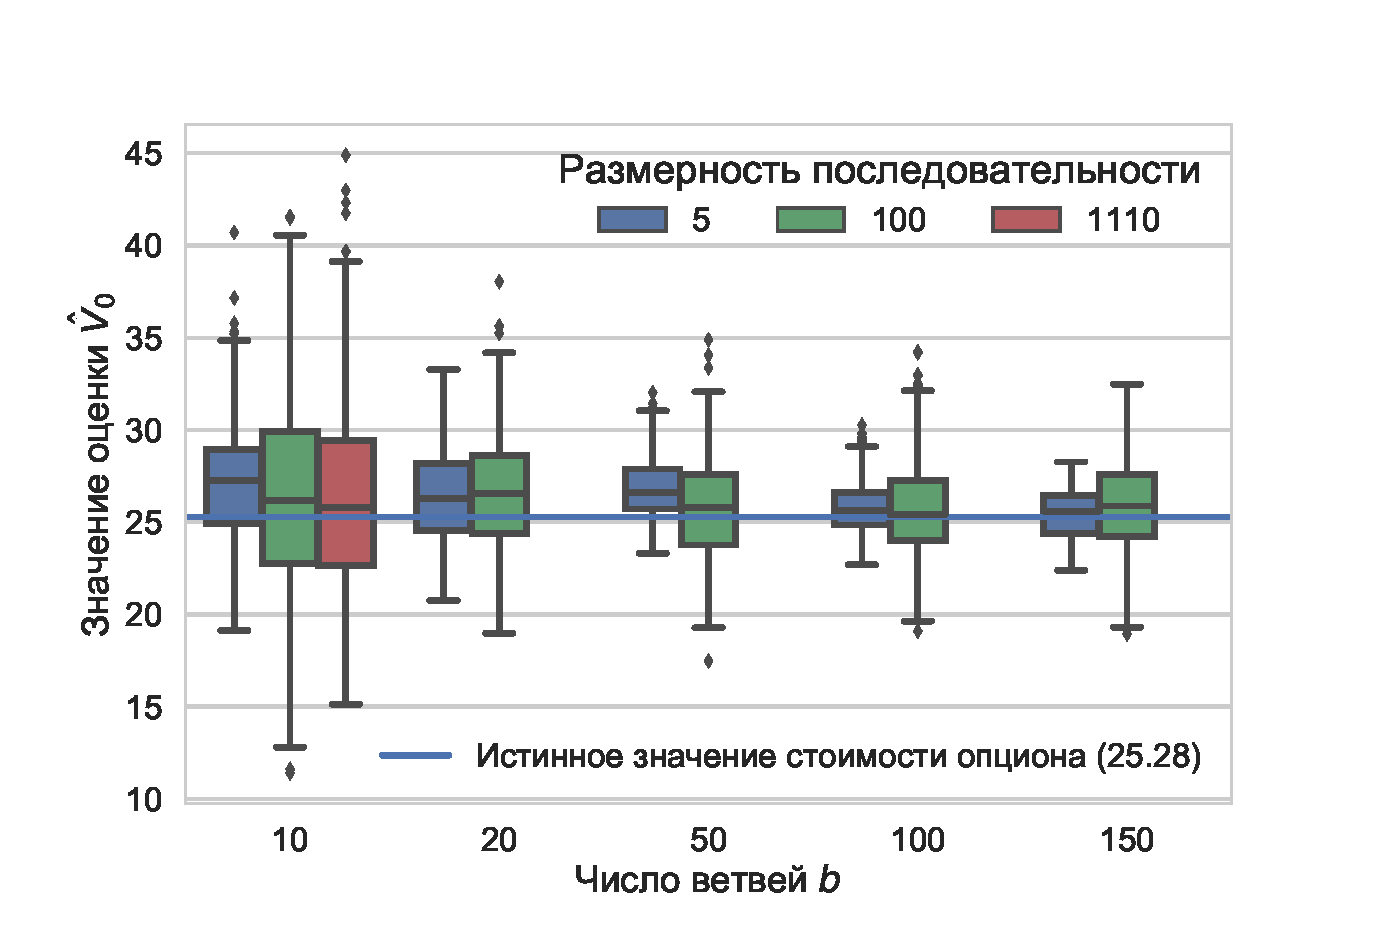
\includegraphics[height=0.75\paperheight]{halton_estimators.eps}
		\caption{Оценки рандомизированными квазислучайными последовательностями}
		% \footnotesize Опцион на 5 независимых базовых активов с $r = 5\%, \delta = 10\%, \sigma = 20\%$. Платёжная функция $h_t(X_t) = \left(\max(X_t) - K\right)^+, X_t\in \mathbb R^5$. Начальная цена каждого из активов $S_0 = 100$, цена страйк $K = 100$, опцион выписан на $T=3$ года. Опцион имеет 4 момента исполнения: в $0, T/3, 2T/3$ и $T$. Вычисления методом случайных деревьев.
		\label{fig:halton_estimators}
	\end{figure}
	\end{frame}	

	\begin{frame}
	\frametitle{Сравнение рандомизированного квази Монте-Карло и обычного Монте-Карло} 
	Отклонения от среднего для квази Монте-Карло значимо меньше, чем для обычного Монте-Карло
	\begin{figure}[h]
	    \centering
		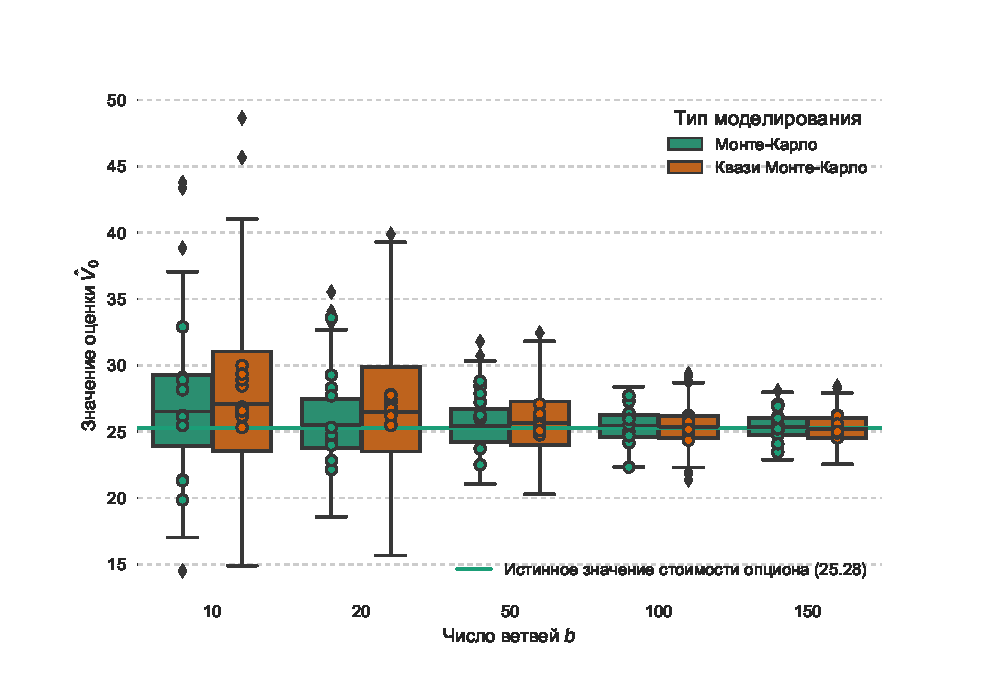
\includegraphics[height=0.65\paperheight]{quasi_vs_common_mc.eps}
		\caption{Сравнение рандомизированной квазислучайной последовательности и стандартного метода}
		% \footnotesize Опцион на 5 независимых базовых активов с $r = 5\%, \delta = 10\%, \sigma = 20\%$. Платёжная функция $h_t(X_t) = \left(\max(X_t) - K\right)^+, X_t\in \mathbb R^5$. Начальная цена каждого из активов $S_0 = 100$, цена страйк $K = 100$, опцион выписан на $T=3$ года. Опцион имеет 4 момента исполнения: в $0, T/3, 2T/3$ и $T$. Вычисления методом случайных деревьев.
		\label{fig:quasi_vs_common_mc}
	\end{figure}
	\end{frame}

	\begin{frame}
	\frametitle{Оставшиеся задачи} 
	% По мере убывания вероятности выполнения:
	\begin{enumerate}
		% \item Использовать рандомизированный квази Монте-Карло для снижения дисперсии оценки. 
		\item Сравнить с другими методами снижения размерности
		\item Сравнить поведение в разных методах оценки
	\end{enumerate}
	\end{frame}
% section results (end)

\end{document}